\chapter{Attacco Denial of Service}
L'attacco di tipo \gls{dos} consiste nel rendere non disponibili servizi offerti da computer o altri
dispositivi \cite{dos-definition}. Questo avviene esasperando di richieste la macchina o infrastruttura che viene scelta come
vittima.

\section{Vulnerabilità nelle reti cellulari}
Le reti cellulari non sono esenti da questo tipo di attacchi, anzi, sono uno degli obiettivi più ambiti e sopratutto difficile da risolvere
poichè le vulnerabilità che sfruttano sono spesso organiche nell'architettura della rete.
Sono diversi i componenti che possono essere vulnerabili a un attacco DOS in una rete cellulare, gli obiettivi identificati come ottimi sono quelli
che comportano un maggior utilizzo delle risorse della rete.\\
Nelle prossime sezioni verranno illustrate le principali metodologie per fare un attacco di tipo \gls{dos} alle reti cellulari\cite{4g-dos-recap}.

\clearpage

\subsection{Radio Jamming}
Il \textit{Radio Jamming} è una tipologia di attacco \textit{Denial of Service} che consiste nel disturbare il segnale cellulare emettendo delle onde radio.
La realizzazione di questo tipo di attacco è molto semplice, basta procurarsi un trasmettitore che invia segnali ad alta energia nella banda cellulare di riferimento.\\
Un miglioramento del classico \textit{radio jamming} è lo \textit{smart jamming} che consiste nel saturare uno o più canali di comunicazione della rete. Questo fa sembrare 
il \textit{network} non disponibile a tutti gli utenti collegati a quella determinata cella.
\begin{figure}[h]
    \centering
    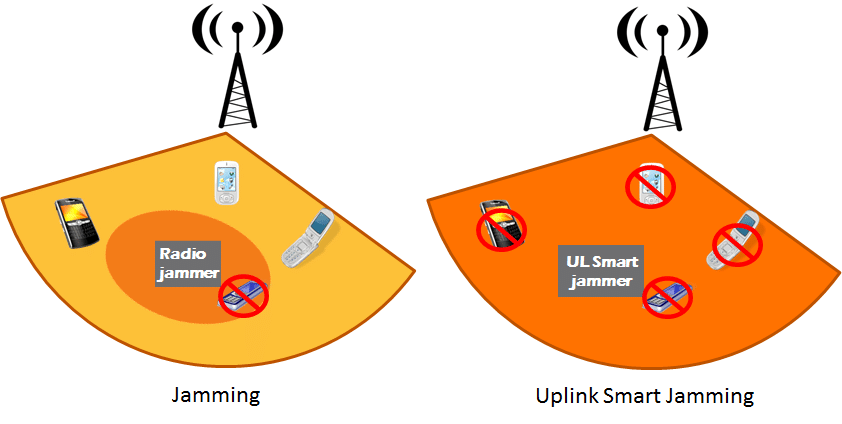
\includegraphics[width=0.6\textwidth]{images/dos-jamming.png}
    \caption{\textit{Radio} e \textit{smart jamming}\cite{4g-dos-recap}}
\end{figure}\\

\subsection{Vulnerabilità di sistema}
Un altro classico modo per creare un interruzione di sistema in una rete cellulare è sfruttando le classiche vulnerabilità che si presentano spesso in qualsiasi tipo di computer.
Questo ovviamente perchè tutta l'architettura di una rete cellulare non è altro che \textit{server} con specifiche particolari.

\subsection{Botnet}
Questa è sicuramente una delle tipologie più diffuse, ed è modo con cui si realizzano i \gls{ddos}. L'attaccante, in questo caso, dispone del controllo di 
un grande numero di dispositivi infettati da \textit{malware} che possono essere attivati da lui per esasperare di richieste un determinato servizio.
\begin{figure}[h]
    \centering
    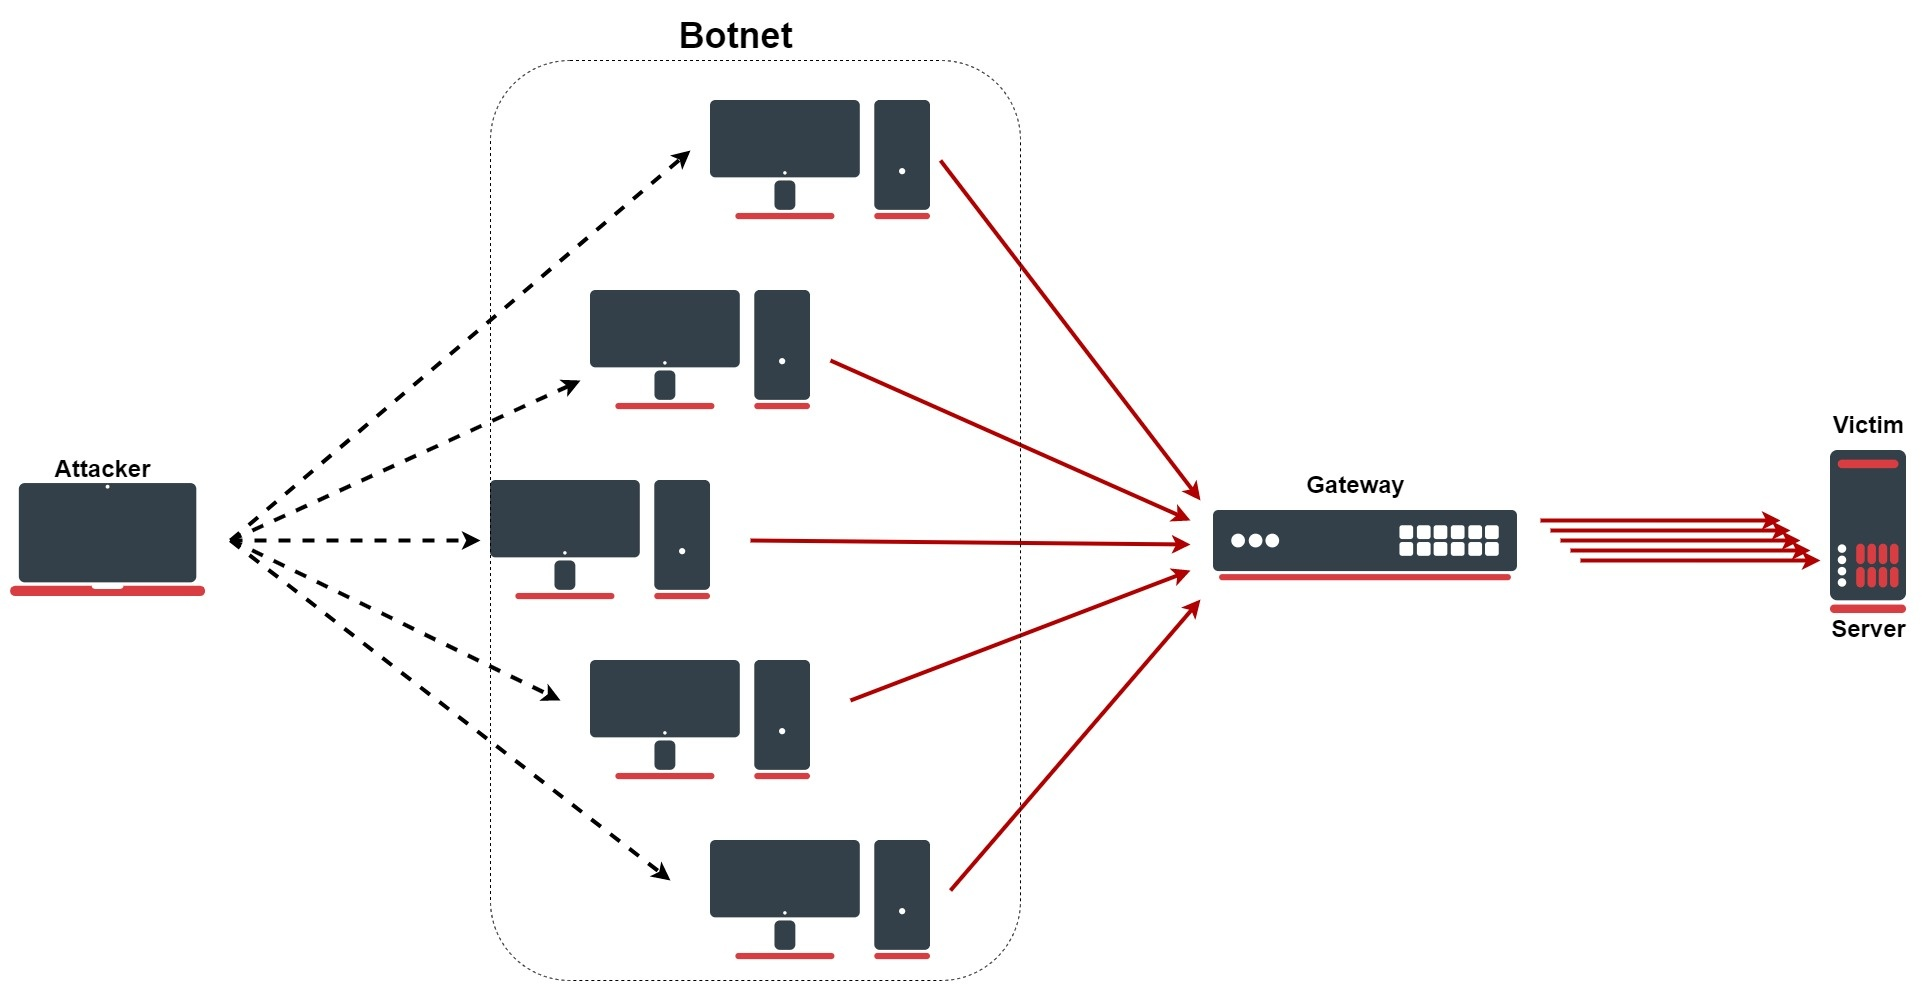
\includegraphics[width=0.5\textwidth]{images/ddos.jpg}
    \caption{\textit{Distributed Denial of Service}}
\end{figure}\\

\subsection{Autenticazione}
Questo è uno degli attacchi più pericolosi poichè le vulnerabilità che sfrutta sono molto difficile da risolvere dato che sono intrinseche nell'architettura del sistema.
È la tipologia di vulnerabilità che è stata scelta per confrontare la sicurezza dell'architettura 5G con quelle precedenti.
Il suo funzionamento si basa sull'esasperare di richieste di autenticazione i sistemi identificativi delle reti cellulari, che solitamente 
sono i componenti con più traffico della rete come la HLR nelle reti 2G/3G.\\
Questa vulnerabilità si trova nel meccanismo di autenticazione dei dispositivi denominato \gls{aka} dove un dispositivo
non autenticato forza delle computazioni all'interno del \textit{core network} che consumano più risorse della richiesta stessa\cite{umts-dos}.
Ad aumentare la pericolosità di questa vulnerabilità è la possibilità di creare computazioni nel \textit{core network} senza essere effettivamente autenticati, e quindi 
senza disporre di una \gls{sim} valida. Questa tipologia di attacchi, definiti come SIM-less, verranno presi come riferimento per sfruttare questa vulnerabilità come illustrato per le 
reti \gls{gsm}\cite{gsm-dos-simless} e \gls{umts}\cite{umts-dos}.



\section{Misurazione}
Per capire quale componente della rete sia il più vulnerabile a un attacco \gls{dos} si devono fare delle misurazioni sui vari componenti del \textit{network}.
In questo modo è possibile capire in quale punto si possono creare dei rallentamenti o \textit{bottleneck} dovuti a un sovraffollamento di richieste.\\
In \cite{measuring-dos} vi è una dettagliata spiegazione di come procedere con queste misurazioni e sopratutto come quantificare il numero di dispositivi che 
servono all'attaccante per completare l'attacco con successo.\\
Solitamente le statistiche riguardo alle prestazioni dei componenti del \textit{network} non sono direttamente fornite dagli operatori telefonici quindi bisogna 
basarsi sui tempi di risposta. Per esempio, l'immagine seguente mostra i tempi di risposta della \gls{hlr} in una rete \gls{umts} al comando \textit{location updates}.
\begin{figure}[h]
    \centering
    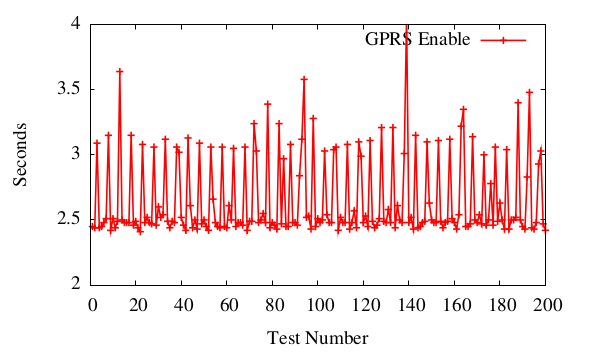
\includegraphics[width=0.7\textwidth]{images/hlr-measuring.png}
    \caption{Misurazione tempi di risposta HLR con \textit{location updates}\cite{measuring-dos}}
\end{figure}